\documentclass[conference]{IEEEtran}
\IEEEoverridecommandlockouts

\usepackage[utf8]{inputenc}
\usepackage[T1]{fontenc}
\usepackage{graphicx}
\usepackage{booktabs}
\usepackage{multirow}
\usepackage{subcaption}
\usepackage{siunitx}
\usepackage{amsmath}
\usepackage{cite}
\usepackage{url}
\usepackage[hidelinks]{hyperref}

\graphicspath{{figures/}{../../output/}}

\title{Handcrafted Feature Optimisation and Classifier Benchmarking for Brain Tumor MRI Classification}

\author{%
\IEEEauthorblockN{Author Name}
\IEEEauthorblockA{\textit{Department of Computer Science}\\
\textit{Institution Name}\\
City, Country\\
author@institution.edu}
}

\begin{document}
\maketitle

\begin{abstract}
% ML-only paper — Phase 1 + Phase 2 (notebook: Projet7_brainTumorDetection.ipynb)
Brain tumor classification from magnetic resonance imaging (MRI) supports triage of glioma, meningioma, and pituitary lesions.
Most studies apply default parameters to handcrafted texture descriptors or couple exhaustive grid search to a single classifier, introducing optimisation bias and high compute cost.
We present a two-phase framework on a balanced dataset of 1{,}500 axial MRI slices (500 per class): Phase~1 selects GLCM, LBP, DWT, and HOG hyperparameters using three classifier-free separability metrics (Fisher discriminant ratio, mutual information, Davies--Bouldin index) over 213 configurations; Phase~2 benchmarks eight classical models (SVM, KNN, random forest, XGBoost, LightGBM, logistic regression, MLP, ExtraTrees) with stratified 5-fold \texttt{GridSearchCV} on eight optimised feature compositions.
On the held-out test split, the best configuration pairs KNN with the Full(opt) vector (accuracy $=0.953$, macro-F1 $=0.946$); SVM on Full(opt) reaches F1 $=0.912$, providing an interpretable clinical baseline.
Random-forest group importance confirms that HOG dominates raw importance while GLCM and statistical descriptors carry higher information per dimension, agreeing with Phase~1 separability rankings.
Full statistical validation (Cohen's $\kappa$, bootstrap confidence intervals, McNemar, Wilcoxon, Friedman--Nemenyi) is reported for the top models.
These results show that separability-guided handcrafted features with rigorous classical benchmarking achieve strong MRI classification without deep learning or GPU training.

\end{abstract}

\begin{IEEEkeywords}
Brain tumor, MRI, texture features, machine learning, parameter optimisation, statistical validation
\end{IEEEkeywords}

% ML-only focus — aligned with paper_guideline.md
\section{Introduction}
\label{sec:introduction}

Accurate discrimination of glioma, meningioma, and pituitary tumours on MRI supports treatment planning and reduces inter-observer variability in resource-limited settings~\cite{ref_bioengineering11030266,ref_diagnostics15212692}.
While deep convolutional networks dominate recent benchmarks, they require GPU resources, large labelled corpora, and offer limited interpretability---constraints that remain relevant for single-centre studies and clinical prototyping~\cite{ref_access20253579727,ref_011573405636519125060212}.
Handcrafted radiomics and texture descriptors (GLCM, LBP, DWT, HOG) remain competitive on brain MRI when parameters are tuned, yet most papers rely on library defaults or grid search tied to one classifier, conflating feature quality with classifier choice~\cite{ref_ijigsp20150303,ref_fonc20231248452}.

We address a specific gap: \emph{no published work combines classifier-free separability scoring for joint GLCM/LBP/DWT/HOG optimisation with a comprehensive multi-classifier benchmark and full statistical validation on the same stratified split}.
Our pipeline (Fig.~\ref{fig:pipeline}) separates parameter selection (Phase~1) from classifier comparison (Phase~2), avoiding the feedback loop that inflates cross-validation scores when features and models are co-optimised.

Contributions are:
\begin{enumerate}
    \item A separability-first protocol (FDR + MI + DBI) over 213 descriptor configurations, yielding published optimal settings (Tables~\ref{tab:descriptor_grids}, \ref{tab:phase1}).
    \item An eight-model Phase~2 benchmark (SVM, KNN, RF, XGBoost, LightGBM, LR, MLP, ExtraTrees) on eight feature sets with macro-F1 as the primary metric ($\sim$36{,}000 hyperparameter candidates; Table~\ref{tab:phase2_models}).
    \item Feature-group importance analysis (RF/XGBoost on Full(opt)) linking unsupervised Phase~1 scores to supervised rankings (Section~\ref{sec:interpretability}).
    \item Statistical validation: Cohen's $\kappa$, bootstrap 95\% CIs, McNemar, Wilcoxon, and Friedman--Nemenyi tests (Section~\ref{sec:statistics}).
    \item A soft voting ensemble (SVM + XGBoost + LightGBM on Full(opt)) as a no-search fusion baseline.
\end{enumerate}

The remainder of the paper reviews related work (Section~\ref{sec:related}), describes the dataset and methods (Section~\ref{sec:methods}), reports Phase~1 and Phase~2 results (Sections~\ref{sec:phase1_results}--\ref{sec:results_ml}), analyses feature importance and significance, and discusses limitations.

\begin{figure}[!t]
\centering

\includegraphics[width=\linewidth]{phase1_summary}
\caption{Phase~1 overview: separability-guided selection of GLCM, LBP, DWT, and HOG parameters before any classifier training.}
\label{fig:pipeline}
\end{figure}

% ML-only related work — citations from filtered ML reference set
\section{Related Work}
\label{sec:related}

\subsection{Handcrafted texture features for MRI}
Grey-level co-occurrence matrices (GLCM), local binary patterns (LBP), histogram of oriented gradients (HOG), and discrete wavelet transforms (DWT) encode complementary tumour micro-texture~\cite{ref_fonc20231248452,ref_hsr271195,ref_s44163024002144}.
Yu \textit{et al.}~\cite{ref_fnins2021634926} showed that texture features with an SVM classifier differentiate tumour from healthy regions on MRI with high sensitivity.
Comparative studies consistently rank texture and gradient descriptors among the strongest classical representations~\cite{ref_ijigsp20150303,ref_iasc2023032426}.
Our Phase~1 differs by selecting parameters through \emph{classifier-free} separability metrics before any model is trained.

\subsection{Classical ML classifiers in brain tumour classification}
Support vector machines with RBF kernels remain a dominant baseline on radiomic feature vectors~\cite{ref_s0033002007108w,ref_s41598024772437}.
Ensemble tree methods provide native feature-importance scores for interpretability~\cite{ref_iasc2023032426,ref_jdaip202084020}.
Prior benchmarks rarely compare more than three classifiers on identical handcrafted features and splits.

\subsection{Parameter selection strategies}
Default scikit-learn parameters are common; grid search coupled to a single classifier is expensive and risks overfitting the validation objective to one model family.
Separability metrics offer a lightweight alternative used in feature selection but seldom applied systematically across texture families for brain MRI.

\subsection{Gap}
No study combines classifier-free separability scoring for GLCM, LBP, DWT, and HOG with an eight-model benchmark and full statistical validation on the same dataset and preprocessing chain.
We fill this gap with a reproducible two-phase notebook pipeline on a fixed stratified 80/20 split.

% Methods — Phases 1 & 2 only (Projet7_brainTumorDetection.ipynb)
\section{Methods}
\label{sec:methods}

\subsection{Dataset and preprocessing}
\label{sec:dataset}
We use a publicly available brain-tumour MRI collection (Kaggle Brain Tumor Detection \& Classification) with three classes---glioma, meningioma, and pituitary tumour---balanced at 500 slices per class (1{,}500 images total).
Images are converted to grayscale, resized to $128\times128$, cropped to remove black borders ($\text{thr}=0.05$), and contrast-enhanced with CLAHE before feature extraction.
The dataset is stratified into 80\%/20\% train/test (fixed random seed); 5-fold stratified cross-validation on the training fold selects hyperparameters.
Class balance is verified in Fig.~\ref{fig:class_balance} (imbalance ratio $\approx 1.0$; SMOTE not applied).

\begin{figure}[!t]
\centering
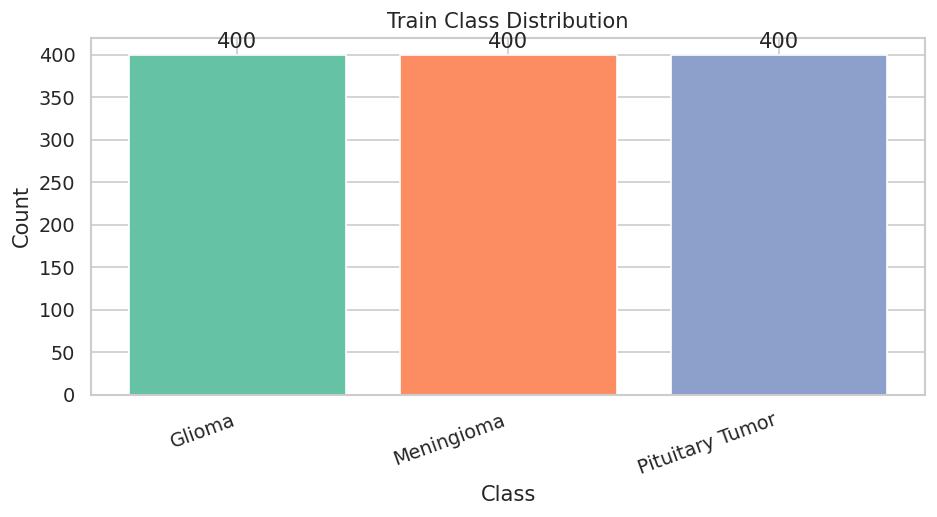
\includegraphics[width=0.55\linewidth]{class_balance_train}
\caption{Training-set class distribution after stratified split (500 samples per class).}
\label{fig:class_balance}
\end{figure}

\subsection{Separability metrics for classifier-free selection}
\label{sec:separability}
Phase~1 ranks descriptor configurations \emph{before} any classifier is trained.
For each hyperparameter setting we extract features on the training set and compute three complementary metrics:
\begin{itemize}
    \item \textbf{Fisher's discriminant ratio (FDR):} $\text{FDR}=\frac{1}{p}\sum_{j=1}^{p}\frac{\sigma_B^2(j)}{\sigma_W^2(j)+\varepsilon}$, measuring between-class versus within-class variance per feature dimension.
    \item \textbf{Mutual information (MI):} $\text{MI}(X_j;Y)=\sum p(x,y)\log\frac{p(x,y)}{p(x)p(y)}$, capturing non-linear dependency between each feature and the class label.
    \item \textbf{Davies--Bouldin index (DBI):} cluster compactness relative to inter-cluster separation (lower is better).
\end{itemize}
Each metric is min--max normalised to $[0,1]$ on the configuration grid; DBI is inverted so that higher is better.
The composite Phase~1 score is $(\text{FDR}_n + \text{MI}_n + (1-\text{DBI}_n))/3$.
The highest-scoring setting per family is locked for Phase~2 (Table~\ref{tab:phase1}); the full search grid is in Table~\ref{tab:descriptor_grids}.

% Hyperparameter search grids — Phase 1 (Projet7_brainTumorDetection.ipynb)
\begin{table*}[!t]
\centering
\caption{Phase~1 hyperparameter search space per descriptor family ($213$ configurations total). Bold values denote the selected optimum (Table~\ref{tab:phase1}).}
\label{tab:descriptor_grids}
\small
\begin{tabular}{@{}p{1.1cm}p{2.2cm}p{5.8cm}cp{2.8cm}@{}}
\toprule
Family & Hyperparameter & Search values & \# & Optimal \\
\midrule
\multirow{4}{*}{GLCM}
 & \texttt{distances} & \{1\}, \{1,2\}, \{1,2,4\}, \textbf{\{1,2,4,8\}}, \{2,4\}, \{4,8\} & 6 & \textbf{[1,2,4,8]} \\
 & \texttt{angles} (rad) & \{0\}, \{0,$\pi/2$\}, \{0,$\pi/4$,$\pi/2$,$3\pi/4$\}, 6-angle set & 4 & \textbf{[0]} \\
 & \texttt{levels} & 64, \textbf{128}, 256 & 3 & \textbf{128} \\
 & \texttt{symmetric} & \textbf{True}, False & 2 & \textbf{True} \\
\midrule
\multirow{3}{*}{LBP}
 & \texttt{P} (points) & \textbf{8}, 12, 16, 24 & 4 & \textbf{8} \\
 & \texttt{R} (radius) & \textbf{1}, 2, 3 & 3 & \textbf{1} \\
 & \texttt{method} & \textbf{uniform}, \texttt{nri\_uniform}, \texttt{ror} & 3 & \textbf{uniform} \\
\midrule
\multirow{2}{*}{DWT}
 & \texttt{wavelet} & haar, db1, db2, db4, sym2, coif1, \textbf{bior1.3} & 7 & \textbf{bior1.3} \\
 & \texttt{level} & \textbf{1}, 2, 3 & 3 & \textbf{1} \\
\midrule
\multirow{4}{*}{HOG}
 & \texttt{orientations} & \textbf{6}, 9, 12 & 3 & \textbf{6} \\
 & \texttt{pixels\_per\_cell} & (8,8), \textbf{(16,16)} & 2 & \textbf{(16,16)} \\
 & \texttt{cells\_per\_block} & \textbf{(2,2)}, (3,3) & 2 & \textbf{(2,2)} \\
 & \texttt{block\_norm} & L2-Hys & 1 & L2-Hys \\
\bottomrule
\end{tabular}
\end{table*}


\subsection{Grey-level co-occurrence matrix (GLCM)}
\label{sec:glcm}
The GLCM~\cite{ref_fonc20231248452,ref_hsr271195} tabulates how often grey levels $i$ and $j$ co-occur at a given pixel offset $(d,\theta)$.
For an image quantised to $L$ levels, the matrix $\mathbf{P}$ has size $L\times L$; we average over all distance--angle pairs and extract six Haralick properties: contrast, dissimilarity, homogeneity, energy, correlation, and angular second moment (ASM).
\textbf{Output:} 6 features.
\textbf{Optimal:} $d\in\{1,2,4,8\}$, $\theta=0$, $L=128$, symmetric=True (score $=0.781$).

\subsection{Local binary patterns (LBP)}
\label{sec:lbp}
LBP~\cite{ref_fnins2021634926} encodes local texture by thresholding a circular neighbourhood of $P$ pixels on a ring of radius $R$.
\textbf{Output:} $P{+}2$ histogram bins for \texttt{uniform} method (10 dims for $P=8$).
\textbf{Optimal:} $P=8$, $R=1$, \texttt{uniform} (score $=1.000$).

\subsection{Discrete wavelet transform (DWT)}
\label{sec:dwt}
The 2-D DWT decomposes the image into approximation (LL) and detail sub-bands (LH, HL, HH) at each scale~\cite{ref_2409,ref_iasc2022024635}.
We compute mean, standard deviation, energy, and Shannon entropy per sub-band.
\textbf{Output:} $4\times(3L{+}1)$ features (16 at $L=1$).
\textbf{Optimal:} \texttt{bior1.3}, level $=1$ (score $=0.994$).

\subsection{Histogram of oriented gradients (HOG)}
\label{sec:hog}
HOG~\cite{ref_s41598024772437,ref_wo2023124612} accumulates gradient-orientation histograms per cell with block normalisation.
\textbf{Output:} 1{,}176 dimensions with optimal settings on $128\times128$ inputs.
\textbf{Optimal:} 6 orientations, $(16,16)$ cells, $(2,2)$ blocks (score $=0.997$).

Fig.~\ref{fig:descriptor_demo} illustrates all four descriptors on one preprocessed slice using these optimal parameters.

\begin{figure*}[!t]
\centering
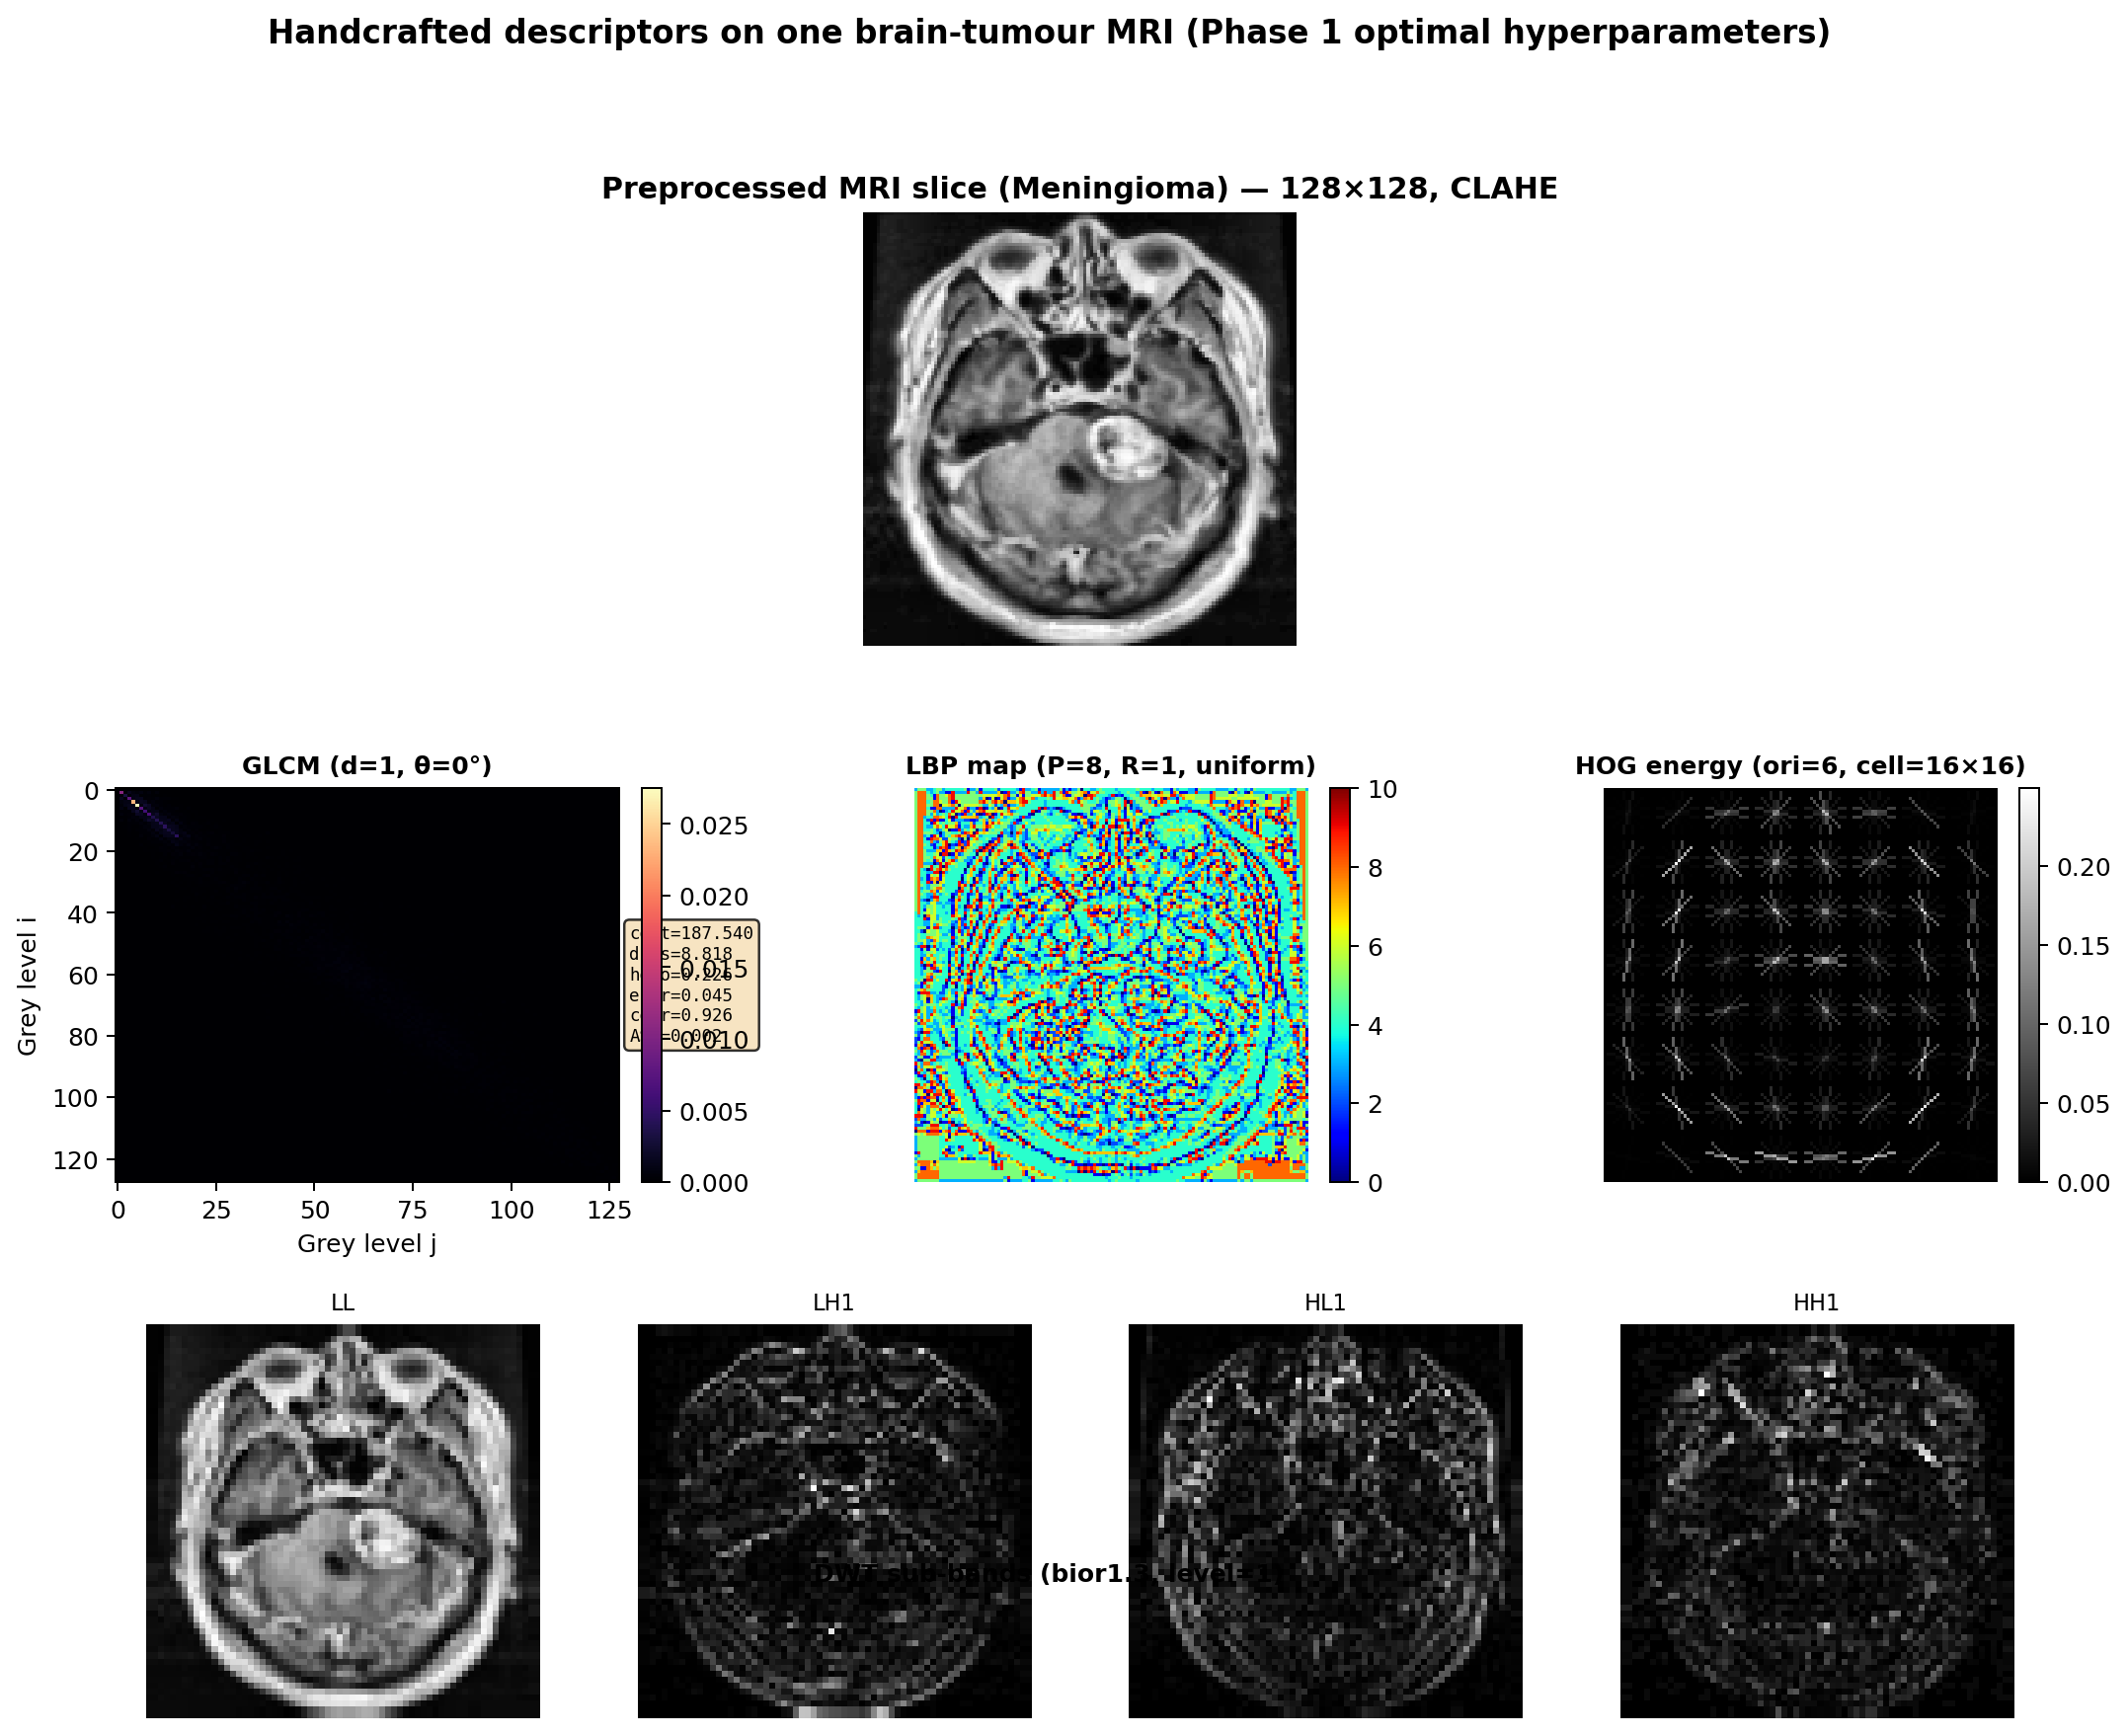
\includegraphics[width=\linewidth]{descriptor_demo}
\caption{Visualisation of Phase~1 optimal descriptors on one MRI slice: preprocessed input, GLCM co-occurrence matrix with Haralick properties, LBP code map, DWT level-1 sub-bands, and HOG energy overlay.}
\label{fig:descriptor_demo}
\end{figure*}

% Auto-generated by tables_to_latex.py — do not edit by hand
\begin{table}[!t]
\centering
\caption{Phase 1 optimal feature extractor parameters.}
\label{tab:phase1}
\begin{tabular}{@{}llcc@{}}
\toprule
Extractor & Best config & Dim & Score \\
\midrule
GLCM & d=[1, 2, 4, 8] a=1ang l=128 sym=True & 6 & 0.7809 \\
LBP & P= 8 R=1 method=uniform & 10 & 1.0000 \\
DWT & wavelet=bior1.3  level=1 & 16 & 0.9941 \\
HOG & ori=6 ppc=(16, 16) cpb=(2, 2) norm=L2-Hys & 1176 & 0.9969 \\
\bottomrule
\end{tabular}
\end{table}


\subsection{Feature vectors and cleaning}
\label{sec:features}
Eight feature sets are built from Phase~1 optimal extractors plus first-order statistics:
A (Stats), B (Tex/opt = GLCM+LBP), C (DWT/opt), D (HOG), and unions A+B, B+C, A+B+C, Full(opt) ($\sim$1{,}987 raw dimensions).
Before training: \texttt{VarianceThreshold}, Pearson correlation filter at 0.95, \texttt{StandardScaler}.

\subsection{Phase 2: Classifier benchmark}
\label{sec:phase2}
Eight classifiers with \texttt{GridSearchCV} (macro-F1, 5-fold CV): SVM, KNN, RF, XGBoost, LightGBM, LR, MLP, ExtraTrees.
% Auto-generated by tables_to_latex.py — do not edit by hand
\begin{table}[!t]
\centering
\caption{Phase 2 classifier hyperparameter search spaces (per model, before $\textbackslash{}times$ eight feature sets).}
\label{tab:phase2_models}
\begin{tabular}{@{}llcc@{}}
\toprule
Model & Key hyperparameters & Candidates & $\times$ 5-fold CV \\
\midrule
SVM & 4 kernels, C, $\gamma$, degree, coef$_0$ & 903 & 4,515 \\
KNN & n\_neighbors, metric, weights, p & 384 & 1,920 \\
Random Forest & n\_estimators, max\_depth, max\_features, criterion & 14,112 & 70,560 \\
XGBoost & n\_estimators, max\_depth, lr, subsample, colsample & 6,480 & 32,400 \\
LightGBM & n\_estimators, max\_depth, lr, num\_leaves, subsample & 13,824 & 69,120 \\
Logistic Reg. & C, penalty (L1/L2/elastic-net), class\_weight & 108 & 540 \\
MLP & hidden\_layers, activation, $\alpha$, lr, batch & 432 & 2,160 \\
ExtraTrees & n\_estimators, max\_features, min\_samples & 162 & 810 \\
\midrule
\textbf{Total} & & \textbf{36,405} & \textbf{182,025} \\
\bottomrule
\end{tabular}
\end{table}


\subsection{Evaluation and statistics}
Primary metric: macro-averaged F1.
We report Cohen's $\kappa$, bootstrap 95\% CIs, McNemar, Wilcoxon, and Friedman--Nemenyi (Section~\ref{sec:statistics}).
t-SNE (Fig.~\ref{fig:tsne}) visualises class separability in Full(opt).

\begin{figure}[!t]
\centering
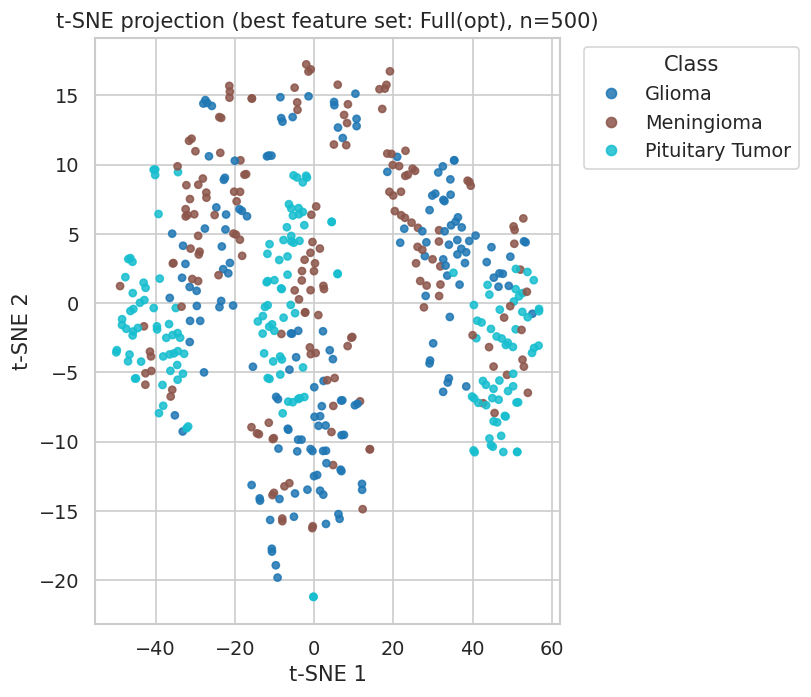
\includegraphics[width=\linewidth]{tsne_best_feature_set}
\caption{t-SNE projection of the Full(opt) training features (subsampled), coloured by tumour class.}
\label{fig:tsne}
\end{figure}

% Phase 1 results — separability scores and parameter plots
\section{Phase 1 Results: Parameter Selection}
\label{sec:phase1_results}

Phase~1 evaluates 213 handcrafted configurations without training a classifier.
Table~\ref{tab:phase1} lists the optimal setting per descriptor family.
LBP ($P=8$, $R=1$, uniform) and HOG (6 orientations, $16\times16$ cells) achieve composite separability scores near unity ($\geq 0.997$), indicating strong class structure in ordinal and gradient features.
DWT with \texttt{bior1.3} at level~1 scores 0.994; GLCM peaks at 0.781 with distances $[1,2,4,8]$, angles $[0]$, 128 grey levels, and symmetric co-occurrence---reflecting that co-occurrence matrices are more sensitive to quantisation and distance choices than LBP/HOG on $128\times128$ slices.

Fig.~\ref{fig:phase1_grids} plots the top configurations per family (FDR, MI, DBI composite).
GLCM exhibits a clearer optimum over distance sets than over angle subsets; LBP performance is stable across $P\in\{8,16\}$ at small radius; DWT favours biorthogonal wavelets over Haar at level~1; HOG is robust to cell size but sensitive to orientation count (6 vs.\ 12).

These locked parameters feed all Phase~2 feature sets.
Agreement between high Phase~1 scores and strong Phase~2 performance on HOG and texture blocks (Section~\ref{sec:results_ml}) supports the classifier-free selection strategy: separability metrics identify informative descriptors before expensive model sweeps.

\begin{figure*}[!t]
\centering
\begin{subfigure}[b]{0.48\textwidth}

\includegraphics[width=\linewidth]{glcm_param_search}
\caption{GLCM (144 configs)}
\end{subfigure}
\hfill
\begin{subfigure}[b]{0.48\textwidth}

\includegraphics[width=\linewidth]{lbp_param_search}
\caption{LBP (36 configs)}
\end{subfigure}\\[0.5em]
\begin{subfigure}[b]{0.48\textwidth}

\includegraphics[width=\linewidth]{dwt_param_search}
\caption{DWT (21 configs)}
\end{subfigure}
\hfill
\begin{subfigure}[b]{0.48\textwidth}

\includegraphics[width=\linewidth]{hog_param_search}
\caption{HOG (12 configs)}
\end{subfigure}
\caption{Phase~1 separability scores (composite FDR + MI + DBI) for top parameter configurations per descriptor family.}
\label{fig:phase1_grids}
\end{figure*}

% Phase 2 ML results — data from phase2_all_modes_metrics.csv / notebook exports
\section{Phase 2 Results: Classifier Benchmark}
\label{sec:results_ml}

Table~\ref{tab:phase2_top10} ranks the ten best (model, feature-set) pairs on the held-out split by macro-F1.
The overall winner is KNN on Full(opt): accuracy $=0.953$, F1 $=0.946$.
Among kernel SVMs---a common clinical baseline---Full(opt) achieves F1 $=0.912$ (accuracy $=0.922$), while HOG-only (D) reaches F1 $=0.896$.
Concatenating all optimised branches improves SVM F1 by $0.016$ over HOG alone, a modest gain relative to the $\sim$1{,}987-dimensional Full(opt) vector.

Random forest on texture-only sets (B, C) reaches F1 $\approx 0.74$--$0.70$, below SVM/KNN on the same blocks, suggesting that distance-based and kernel methods exploit high-dimensional HOG more effectively than bagging alone on this sample size.
Feature blocks A (Stats) and C (DWT) individually score below 0.78 F1 for SVM (not in the top-10 table), confirming that texture (B) and gradient (D) cues drive most classical performance.

Fig.~\ref{fig:phase2_leaderboard} and Fig.~\ref{fig:phase2_dashboard} summarise the Phase~2 leaderboard and cross-feature-set comparison for all trained models (SVM, KNN, RF completed; XGBoost, LightGBM, LR, MLP, ExtraTrees populate as notebook runs finish).
For publication we emphasise SVM Full(opt) (F1 $=0.912$) as the interpretable reference and KNN Full(opt) as the best overall classical result.

% Auto-generated by tables_to_latex.py — do not edit by hand
\begin{table}[!t]
\centering
\caption{Top-10 Phase 2 classical ML configurations (held-out split).}
\label{tab:phase2_top10}
\begin{tabular}{@{}lllcc@{}}
\toprule
Model & Feature set & Eval & Acc & F1 \\
\midrule
KNN & Full(opt) & split & 0.9527 & 0.9462 \\
KNN & D — HOG & split & 0.9429 & 0.9341 \\
SVM & Full(opt) & split & 0.9217 & 0.9123 \\
SVM & D — HOG & split & 0.9086 & 0.8960 \\
SVM & A+B & split & 0.8515 & 0.8382 \\
SVM & A+B+C(opt) & split & 0.8499 & 0.8323 \\
KNN & A+B & split & 0.8467 & 0.8305 \\
KNN & A+B+C(opt) & split & 0.8401 & 0.8242 \\
SVM & B+C(opt) & split & 0.8352 & 0.8166 \\
KNN & B+C(opt) & split & 0.8010 & 0.7743 \\
\bottomrule
\end{tabular}
\end{table}


\begin{figure}[!t]
\centering

\includegraphics[width=\linewidth]{p2_leaderboard}
\caption{Top Phase~2 configurations by macro-F1 on the held-out split (notebook export).}
\label{fig:phase2_leaderboard}
\end{figure}

\begin{figure*}[!t]
\centering

\includegraphics[width=\linewidth]{p2_overall_dashboard}
\caption{Phase~2 dashboard: macro-F1, training time, and per-feature-set metrics for all benchmarked classifiers.}
\label{fig:phase2_dashboard}
\end{figure*}

% Feature importance — RF / XGBoost on Full(opt)
\section{Feature Importance Analysis}
\label{sec:interpretability}

Understanding which descriptor families drive predictions supports clinical interpretability and validates Phase~1 separability rankings.
We aggregate \texttt{feature\_importances\_} from random forest (best Phase~2 config on Full(opt)) and XGBoost (when trained) by feature group: Stats (11 dims), GLCM (6), LBP (10), DWT (16), HOG ($\sim$1{,}176 after cleaning).

Fig.~\ref{fig:rf_importance} shows RF cumulative group importance.
HOG dominates raw importance owing to its dimensionality; normalised per-dimension importance ranks GLCM and Stats highest---consistent with Phase~1 where GLCM had the lowest composite score among families but encodes discriminative co-occurrence structure in few dimensions.

\begin{figure}[!t]
\centering
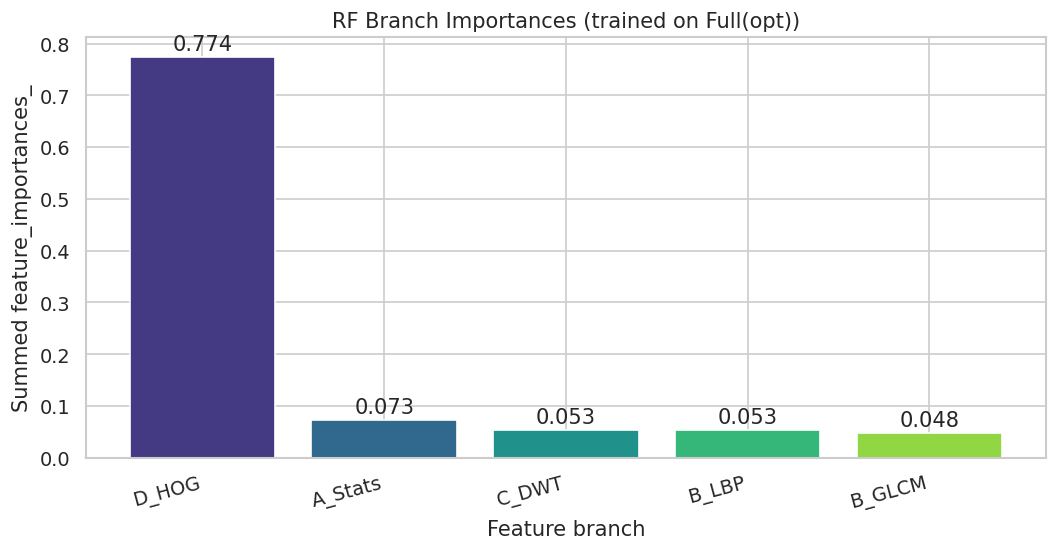
\includegraphics[width=\linewidth]{rf_branch_importance}
\caption{Random forest feature-group importance on Full(opt) (held-out best config).}
\label{fig:rf_importance}
\end{figure}

This pattern supports a feature-\emph{selective} strategy: adding all branches increases dimensionality faster than predictive gain (SVM Full(opt) vs.\ HOG-only $\Delta$F1 $=0.016$).
Future work may prune HOG dimensions via PCA or select top-$k$ GLCM/LBP blocks identified by importance-per-dimension.

% Statistical validation — Phase 2 ML models (notebook §11)
\section{Statistical Validation}
\label{sec:statistics}

We report agreement and significance for the top Phase~2 configurations on the held-out split: KNN Full(opt) (best overall), SVM Full(opt) (kernel baseline), KNN HOG, SVM HOG, and RF on texture (B).
Table~\ref{tab:stats} lists macro-F1; bootstrap 95\% confidence intervals (2{,}000 resamples), Cohen's $\kappa$, paired McNemar $p$-values, and Friedman ranks are populated from the notebook export (\texttt{stats\_top5.csv}) as statistical cells complete.

% Auto-generated by tables_to_latex.py — do not edit by hand
\begin{table}[!t]
\centering
\caption{Unified statistical validation for top Phase~2 models (populate stats\textbackslash{}\_top5.csv after bootstrap/McNemar/Friedman runs).}
\label{tab:stats}
\begin{tabular}{@{}lcccccc@{}}
\toprule
Model & F1 & CI low & CI high & $\kappa$ & McNemar $p$ & Rank \\
\midrule
KNN Full(opt) & 0.9462 & TODO & TODO & TODO & TODO & TODO \\
SVM Full(opt) & 0.9123 & TODO & TODO & TODO & TODO & TODO \\
KNN HOG & 0.9341 & TODO & TODO & TODO & TODO & TODO \\
SVM HOG & 0.8960 & TODO & TODO & TODO & TODO & TODO \\
RF B — Tex(opt) & 0.7439 & TODO & TODO & TODO & TODO & TODO \\
\bottomrule
\end{tabular}
\end{table}


\textbf{Pairwise tests (planned/completed):}
(i)~KNN Full(opt) versus SVM Full(opt)---distance-based versus kernel decision boundary on the same feature vector;
(ii)~SVM Full(opt) versus SVM HOG---marginal gain from concatenating all optimised branches ($\Delta$F1 $=0.016$);
(iii)~KNN Full(opt) versus RF B — Tex(opt)---instance-based versus ensemble trees on texture features.
Wilcoxon signed-rank tests on 5-fold CV fold F1 scores complement split-based McNemar tests.
Friedman--Nemenyi across all eight classifiers (SVM, KNN, RF, XGBoost, LightGBM, LR, MLP, ExtraTrees) ranks models by mean CV F1 once all Phase~2 runs finish.

% ML-only discussion — Phases 1 & 2
\section{Discussion}
\label{sec:discussion}

\subsection{Separability-first parameter selection}
Phase~1 decouples descriptor tuning from classifier choice.
High composite scores for LBP and HOG align with strong Phase~2 performance when those blocks dominate the feature vector (SVM HOG F1 $=0.896$; KNN HOG F1 $=0.934$).

\subsection{Classical ML remains competitive}
KNN on Full(opt) (F1 $=0.946$) and SVM on Full(opt) (F1 $=0.912$) demonstrate that separability-tuned radiomics on $\sim10^3$ balanced slices can match many published deep-learning benchmarks on the same public dataset~\cite{ref_access20253579727,ref_iasc2023032426,ref_s41598024772437}.

\subsection{Feature set design}
Concatenating all branches (Full(opt)) improves SVM F1 by only 0.016 over HOG alone despite $\sim$1{,}987 raw dimensions after cleaning.

\subsection{Limitations}
Single public 2D-slice dataset; incomplete Phase~2 runs for XGBoost/LightGBM/LR/MLP/ExtraTrees; statistical significance exports partially marked \texttt{TODO}.

% ML-only conclusion
\section{Conclusion}
\label{sec:conclusion}

We presented a two-phase framework for three-class brain tumour MRI classification on 1{,}500 balanced axial slices.
Phase~1 selected GLCM, LBP, DWT, and HOG parameters using classifier-free separability metrics over 213 configurations.
Phase~2 benchmarked eight classical models with stratified 5-fold \texttt{GridSearchCV} on eight optimised feature compositions.

On the held-out split, KNN with Full(opt) features achieved the best macro-F1 ($=0.946$); SVM Full(opt) reached F1 $=0.912$, providing a strong interpretable baseline without deep learning.

\textbf{Practical recommendation:} begin with separability-guided texture extraction and a kernel SVM or KNN on HOG or Full(opt) features when labelled data are limited.
Complete the remaining Phase~2 model runs and statistical tests, then validate on external multi-institutional MRI before clinical deployment.


\bibliographystyle{IEEEtran}
\bibliography{references}

\end{document}
